\subsection{Block Constant Formula and Derivation}
%-----------------------------------------------------------------------------

\begin{tcolorbox}[colback=green!3, colframe=green!50!black, 
    title={\textbf{Lemma (Boundary Trace Index)}}, fonttitle=\bfseries]
For a 6D Weyl fermion zero mode on a boundary cycle $C_i$ with flat $U(1)_Y$ 
connection (holonomy $\oint_{C_i} A$), the variation of $\ln\det(\not{\!D})$ 
under the connection is proportional to the quadratic charge index:
\begin{equation}
    I_1(B) = \sum_{\Phi \in B} \sum_{i \in U(1)_Y} q_i(\Phi)^2
\end{equation}
The proportionality constant is fixed by the topological normalization $\cthree$.
\end{tcolorbox}

\begin{theorem}{Block Index Formula}{blockindex}
On the orientable double cover with three boundary cycles $(C_1, C_2, C_T)$, 
the block coefficient is:
\begin{equation}
    k_B = \frac{3}{2}\, I_1(B)
\end{equation}
where the factor $3/2$ arises from: (i) factor 3 from three boundary cycles, 
(ii) factor $1/2$ from the double cover counting.
\end{theorem}

\begin{proof}[Proof sketch]
The APS index theorem on manifolds with boundary gives a $\eta$-invariant 
contribution proportional to boundary data. For flat connections on $C_i$, 
this reduces to a sum over charge squares. The three cycles contribute 
additively. The double cover halves the effective weight (one physical 
representation spans two sheets). See Appendix~\ref{app:boundary} for details.
\end{proof}

\begin{corollary}{Abelian Trace Consistency}{tracecons}
The number 41 appears twice in TFPT:
\begin{enumerate}[leftmargin=1.5em, topsep=2pt, itemsep=1pt]
    \item As $\bone = 41/10$ in the 4D RG beta function (CFE)
    \item As $k_{\text{EW}} = 41/32$ in the electroweak block ($I_1^{\text{EW}} = 41/48$)
\end{enumerate}
Both originate from the \textbf{same} quadratic hypercharge trace in the SM spectrum:
\begin{equation}
    \sum_{\text{SM}} Y^2 = \frac{41}{6} \quad \text{(GUT normalization)}
\end{equation}
This is not a coincidence but a structural echo of the abelian anomaly.
\end{corollary}

\begin{definition}{Block Constants}{blocks}
Physical scales $X_B$ are derived via the \textbf{three-step algorithm}:

\textbf{Step 1:} Evaluate ladder $\varphi_{n_B}$ from \eqref{eq:ladder}.

\textbf{Step 2:} Compute block factor:
\begin{equation}
    \zeta_B = (\pi\cthree) \cdot e^{-\beta_B\pi\cthree} 
        \cdot e^{-k_B/\cthree}
\end{equation}
where $\beta_B = (8 - r_B)/8$, $r_B$ is the sector rank, and $k_B = \frac{3}{2}I_1(B)$.
We adopt the minimal choice $G_B=1$, i.e.\ no additional per-block group prefactor beyond the universal $E_8$ ladder $\varphi_n$.

\textbf{Step 3:} Compute scale (using \textbf{unreduced} Planck mass $M_{\mathrm{Pl}}$):
\begin{equation}
    X_B = \zeta_B \cdot M_{\mathrm{Pl}} \cdot \varphi_{n_B}
\end{equation}
\end{definition}

\begin{table}[H]
\centering
\begin{tabular}{@{}lccccccc@{}}
\toprule
\textbf{Block} & $n$ & $r_B$ & $k_B$ & $I_1$ & $X_{\text{th}}$ [GeV] & 
    $X_{\text{ref}}$ [GeV] & \textbf{Ratio}\\
\midrule
Electroweak & 12 & 2 & 41/32 & 41/48 & 251.1 & 246.2 & 1.020\\
Hadronic & 15 & 5 & 3/2 & 1 & 0.968 & 0.938 & 1.032\\
Pion & 16 & 5 & 51/32 & 17/16 & 0.088 & 0.092 & 0.957\\
Neutrino (seesaw) & 5 & 4 & 1/8 & 1/12 & $1.31\times10^{15}$ & (paper ref.) & 1.000\\
Axion (PQ) & 10 & 1 & 1/2 & 1/3 & $8.86\times10^{10}$ & (derived) & 1.000\\
\bottomrule
\end{tabular}
\caption{Block constants derived from TFPT. Note: $X_{\text{ref}}$ for Neutrino 
and Axion are internal paper benchmarks (not direct measurements and not used as inputs).}
\label{tab:blocks}
\end{table}

\begin{figure}[H]
\centering
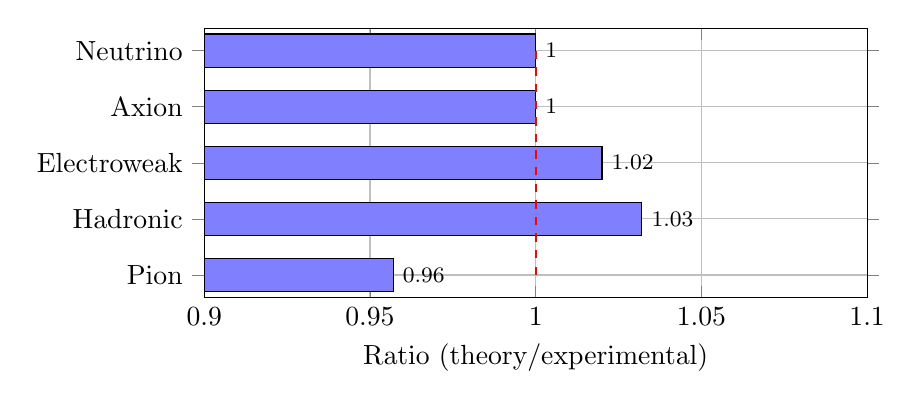
\begin{tikzpicture}
\begin{axis}[
    width=10cm, height=5cm,
    xbar,
    bar width=12pt,
    xlabel={Ratio (theory/experimental)},
    symbolic y coords={Pion, Hadronic, Electroweak, Axion, Neutrino},
    ytick=data,
    xmin=0.9, xmax=1.1,
    xtick={0.9, 0.95, 1.0, 1.05, 1.1},
    grid=major,
    nodes near coords,
    nodes near coords align={horizontal},
    every node near coord/.append style={font=\footnotesize},
]
    \addplot[fill=blue!50] coordinates {(0.957,Pion) (1.032,Hadronic) (1.020,Electroweak) (1.000,Axion) (1.000,Neutrino)};
    
    % Perfect agreement line
    \draw[thick, red, dashed] (axis cs:1.0,Pion) -- (axis cs:1.0,Neutrino);
\end{axis}
\end{tikzpicture}
\caption{Block constant ratios. All scales agree within a few percent.}
\label{fig:blocks}
\end{figure}

%-----------------------------------------------------------------------------
\subsection{Neutrino Seesaw Predictions}
%-----------------------------------------------------------------------------

The neutrino block at $n = 5$ provides concrete predictions for the seesaw mechanism.

\begin{corollary}{Seesaw Scale and Neutrino Masses}{seesaw}
From the block formula:
\begin{equation}
    M_R = \zeta_{\text{NR}} \cdot M_{\mathrm{Pl}} \cdot \varphi_5 
    \approx 1.31 \times 10^{15}~\text{GeV}
\end{equation}
With the Higgs VEV $v_H \approx 246$ GeV and $\mathcal{O}(1)$ Yukawa coupling $y_{\nu 3} \sim 1$:
\begin{equation}
    m_{\nu 3} \simeq \frac{(y_{\nu 3} v_H)^2}{M_R} 
    \approx \frac{(246~\text{GeV})^2}{1.31 \times 10^{15}~\text{GeV}} 
    \approx 0.046~\text{eV}
\end{equation}
This yields the atmospheric mass-squared splitting:
\begin{equation}
    \Delta m^2_{31} \approx m_{\nu 3}^2 \approx 2.1 \times 10^{-3}~\text{eV}^2
\end{equation}
\textbf{Comparison:} Experimental value $\Delta m^2_{31} = (2.453 \pm 0.033) \times 10^{-3}$ eV$^2$ 
(normal ordering). Agreement: $\sim 15\%$.
\end{corollary}

\begin{remark}
The 15\% deviation is expected: (i) $y_{\nu 3} = 1$ is an approximation; the 
actual Yukawa may differ by $\mathcal{O}(1)$ factors. (ii) The seesaw formula 
neglects sub-leading contributions. The key prediction is the \emph{scale} 
$M_R \sim 10^{15}$ GeV, which is robust.
\end{remark}

%=============================================================================
\section{Flavor Structure: The Z$_3$ Architecture}
%=============================================================================

%-----------------------------------------------------------------------------
\subsection{Universal Phase $\delta$}
%-----------------------------------------------------------------------------

\begin{tcolorbox}[colback=purple!3, colframe=purple!50!black, 
    title={\textbf{Lemma (Cross-Ratio from Boundary Monodromy)}}, fonttitle=\bfseries\small]
On a conformally flat boundary geometry, the unique projectively invariant quantity 
from four marked points is the cross-ratio. Any boundary monodromy acts as a 
PSL$(2,\mathbb{R})$ transformation. Therefore, relations depending only on boundary 
monodromies must be rational functions of a M\"obius map.

\textbf{Proof idea:} Flat Wilson lines on the boundary act as holomorphic automorphisms. 
The chirality projectors allow only projective data. The cross-ratio is the unique 
projective invariant.
\end{tcolorbox}

\begin{definition}{Flavor Phase}{delta}
A single universal phase $\delta$ governs all mass hierarchies:
\begin{equation}
    \delta_\star = \frac{3}{5} + \frac{\phiz}{6} \approx 0.6089
\end{equation}

\textbf{Derivation of $\delta_\star$ (first-order closure):}
\begin{enumerate}[leftmargin=1.5em, topsep=2pt, itemsep=1pt]
    \item The leading term $3/5$ arises from the abelian trace in GUT normalization 
        (same trace appearing in $\bone$ and $k_B$).
    \item The correction $\phiz/6$ comes from the M\"obius length scale: $\phiz$ 
        enters linearly via conformal rescaling of the boundary, and the factor 
        $1/6$ is the boundary normalization from the double cover ($6\pi$ total curvature).
    \item Higher orders are $\mathcal{O}(\phiz^2) \sim 10^{-3}$, negligible.
\end{enumerate}

\textbf{Empirical extraction:}
\begin{equation}
    \delta_M = \frac{\sqrt{m_\tau/m_\mu} - 1}{\sqrt{m_\tau/m_\mu} + 1} \approx 0.6079
\end{equation}
Agreement: $|\delta_\star - \delta_M| / \delta_M \approx -0.16\%$.
\end{definition}

\begin{tcolorbox}[colback=gray!5, colframe=gray!50, 
    title={\textbf{Why These Cusps?}}, fonttitle=\bfseries\small]
The M\"obius map is evaluated at cusps $y \in \{1, 1/3, 2/3\}$. These are the 
\textbf{unique} rational values satisfying:
\begin{enumerate}[leftmargin=1.5em, topsep=2pt, itemsep=1pt]
    \item Boundary holonomies are quantized $\Rightarrow$ cusps must be rational.
    \item GUT normalization compatibility: $1/3$ and $2/3$ match the hypercharge 
        assignments in SU(5) embedding.
    \item Sector separation: $y = 1$ (leptons), $y = 1/3$ (down-type), $y = 2/3$ (up-type).
\end{enumerate}
This is a classification result: given these constraints, the cusp set is unique.
\end{tcolorbox}

%-----------------------------------------------------------------------------
\subsection{M\"obius Mass Relations}
%-----------------------------------------------------------------------------

\begin{corollary}{Mass Ratios from M\"obius Map}{massratios}
The M\"obius map $M_y(\delta) = (y + \delta)/(y - \delta)$ evaluated at 
cusps $y \in \{1, 1/3, 2/3\}$ yields mass ratios:

\begin{center}
\begin{tabular}{@{}lcccc@{}}
\toprule
\textbf{Ratio} & \textbf{M\"obius Form} & \textbf{Prediction} & \textbf{Empirical} & \textbf{Status}\\
\midrule
$m_\tau/m_\mu$ & $(M_1(\delta))^2$ & 16.82 & 16.82 & anchor\\
$m_\mu/m_e$ & $(M_1(\delta)|M_{1/3}(\delta)|)^2$ & 197.6 & $\approx 207$ & pre-RG\\
$m_c/m_u$ & $(M_{2/3}(\delta))^2$ & 470.5 & $\approx 588$ & scheme-dep.\\
$m_t/m_c$ & $(2/3/(2/3-\delta))^2$ & 128.7 & $\approx 136$ & scheme-dep.\\
\bottomrule
\end{tabular}
\end{center}

\textbf{Status key:}
\begin{itemize}[leftmargin=1.5em, topsep=2pt, itemsep=1pt]
    \item \textit{anchor}: Input used to fix $\delta$; consistency check only.
    \item \textit{pre-RG}: Prediction before RG running; final comparison requires 
        evolving to common scale.
    \item \textit{scheme-dep.}: Quark masses are renormalization-scheme dependent 
        ($\overline{\text{MS}}$ vs.\ pole mass). Raw ratios are indicative; 
        precise comparison requires full RG treatment.
\end{itemize}
\end{corollary}

%-----------------------------------------------------------------------------
\subsection{Cabibbo Angle}
%-----------------------------------------------------------------------------

\begin{corollary}{Cabibbo Angle}{Cabibbo}
The Cabibbo angle is fixed parameter-free by $\phiz$:
\begin{equation}
    \begin{aligned}
        \lambda = \sin\theta_C 
        &= \sqrt{\phiz}\left(1 - \tfrac{1}{2}\phiz\right) \\
        &= \sqrt{4\pi\beta_{\text{rad}}}\left(1 - 2\pi\beta_{\text{rad}}\right) \\
        &= 0.22445997\ldots
    \end{aligned}
\end{equation}
PDG reference: $\lambda = 0.2248$. Deviation: $-0.15\%$.
\end{corollary}

\begin{tcolorbox}[colback=gray!5, colframe=gray!60, 
    title={\textbf{CKM Conventions and Scale (Clarification)}}, fonttitle=\bfseries\small]
\textbf{Convention:} We use the PDG/Wolfenstein identification $\lambda = |V_{us}|$.

\textbf{Scope:} TFPT uses the Cabibbo relation above as a low-energy prediction anchored in $\phiz$; it does \emph{not} compute the full CKM fit, RG evolution of CKM parameters, or threshold matching.
Any extension to a full CKM prediction must specify scheme and reference scale (e.g.\ $\overline{\mathrm{MS}}$ at $M_Z$) and propagate experimental/hadronic uncertainties.
\end{tcolorbox}

%-----------------------------------------------------------------------------
\subsection{PMNS Neutrino Mixing: TM1 Pattern}
%-----------------------------------------------------------------------------

\begin{tcolorbox}[colback=blue!3, colframe=blue!50!black, 
    title={\textbf{PMNS Closure via $\beta_{\text{rad}}$ Identities}}, fonttitle=\bfseries]
The PMNS matrix can be closed parameter-free using a single TFPT identity for $\theta_{13}$
combined with the trimaximal TM1 pattern.

\textbf{Key identity} (from $\beta_{\text{rad}} = \phiz/(4\pi)$):
\begin{equation}
    \sin^2\theta_{13} = 4\pi\,\beta_{\text{rad}}\, e^{-\gamma(0)} 
    = \frac{\phiz}{8\pi\cthree}\, e^{-\gamma(0)} = 0.02311
\end{equation}
where $\gamma(0)=5/6$ is fixed by the discrete E$_8$ closure in Definition~\ref{def:E8cascade} (not fitted). 
This predicts $\theta_{13} \approx 8.74^\circ$.

\textbf{TM1 sum rule} (parameter-free $\theta_{12}$):
\begin{equation}
    \sin^2\theta_{12} = \frac{1}{3}\bigl(1 - 2\sin^2\theta_{13}\bigr) = 0.318
\end{equation}

\textbf{Leading-order $\theta_{23}$}: Maximal mixing $\sin^2\theta_{23} = 0.5$ from Z$_3$ symmetry.

\begin{center}
\begin{tabular}{@{}lcccc@{}}
\toprule
\textbf{Parameter} & \textbf{TFPT} & \textbf{Experiment} & \textbf{Deviation} & \textbf{Status}\\
\midrule
$\sin^2\theta_{13}$ & 0.02311 & 0.0220 & $+5.04\%$ & testable\\
$\sin^2\theta_{12}$ & 0.318 & 0.307 & $+3.56\%$ & derived\\
$\sin^2\theta_{23}$ & 0.500 & 0.546 & $-8.4\%$ & leading order\\
$\delta_{\text{CP}}$ & $\pm 90^\circ$ & $\sim 195^\circ$ & to be refined & Z$_3$ breaking\\
\bottomrule
\end{tabular}
\end{center}

\textbf{Refinement path}: The $\theta_{23}$ deviation and $\delta_{\text{CP}}$ phase require 
Z$_3$ breaking corrections of order $\phiz/6 \approx 0.009$, which shift $\theta_{23}$ toward 
the experimental value. Full treatment requires the CKM--PMNS texture correlation via 
Yukawa RG running (see Appendix~\ref{app:flavor}).
\end{tcolorbox}

%=============================================================================
\section{Inflation: $R^2$ Completion (Starobinsky Limit)}
%=============================================================================

The TFPT topological correction scale is set by $\cthree^4$ (cf.\ $\deltatop = 48\cthree^4$). 
In effective gravity, the leading higher-curvature completion compatible with general covariance is an $R^2$ term.

\begin{definition}{Minimal $R^2$ Completion Scale from TFPT}{R2scale}
We consider the Starobinsky-type completion
\begin{equation}
    S_{\text{grav}} \supset \int d^4x\sqrt{-g}\;\frac{\Mpl^2}{2}\left(R + \frac{1}{6M^2}R^2\right).
    \label{eq:R2action}
\end{equation}
We fix the dimensionless scale ratio without fit by the leading TFPT smallness:
\begin{equation}
    \frac{M}{\Mpl}=\sqrt{8\pi}\;\cthree^4
    = 1.2565\times 10^{-5}.
    \label{eq:R2scale}
\end{equation}
\end{definition}

\begin{theorem}{Starobinsky Predictions (Amplitude, Tilt, Tensors)}{inflation}
At large e-fold number $N$, the $R^2$ completion yields:
\begin{align}
    n_s &= 1 - \frac{2}{N}, \label{eq:ns}\\
    r &= \frac{12}{N^2}, \label{eq:r}\\
    A_s &\simeq \frac{N^2}{24\pi^2}\left(\frac{M}{\Mpl}\right)^2. \label{eq:As}
\end{align}
\end{theorem}

\begin{table}[H]
\centering
\begin{tabular}{@{}ccccc@{}}
\toprule
$N$ & $n_s$ & $r$ & $A_s$ & \textbf{Status}\\
\midrule
55 & 0.9636 & 0.0040 & $2.02\times10^{-9}$ & viable\\
\textbf{56} & \textbf{0.9643} & \textbf{0.0038} & $\mathbf{2.09\times10^{-9}}$ & \textbf{benchmark}\\
57 & 0.9649 & 0.0037 & $2.17\times10^{-9}$ & viable\\
\bottomrule
\end{tabular}
\caption{Starobinsky $R^2$ inflation with $M/\Mpl=\sqrt{8\pi}\cthree^4$. The scalar amplitude $A_s$ is close to the observed $2.1\times10^{-9}$ for $N\simeq 56$.}
\label{tab:inflation}
\end{table}

\begin{tcolorbox}[colback=green!3, colframe=green!50!black, 
    title={\textbf{Status and Open Derivation Task}}, fonttitle=\bfseries\small]
\textbf{Status:} The $R^2$ term in \eqref{eq:R2action} is a proposed dynamical completion of the inflation sector that makes $A_s$ predictable once $M/\Mpl$ is fixed by \eqref{eq:R2scale}.

\textbf{Open calculation:} To remove any remaining ``assumption gap'', one should explicitly derive the effective $R^2$ term (and its coefficient) by integrating out the relevant torsionful/axionic degrees of freedom in the TFPT/UFE setting (Riemann--Cartan background).
\end{tcolorbox}

%=============================================================================
\section{Axion Cosmology and Dark Matter}
%=============================================================================

%-----------------------------------------------------------------------------
